\documentclass{beamer}
\usetheme{Madrid}
\usecolortheme{seahorse}
\usepackage{graphicx}
\usepackage{amsmath}
\usepackage{hyperref}
\usepackage{caption}
\usepackage{subcaption}

\title{Reservoir Computing: Implementation and Analysis}
\subtitle{Study Oriented Project Seminar}
\author{Vimarsh Shah}
\institute{BITS Pilani, Goa}
\date{April 2025}

\begin{document}

\begin{frame}
  \titlepage
\end{frame}

\begin{frame}{Overview}
  \tableofcontents
\end{frame}

\section{Introduction}
\begin{frame}{Machine Learning Context}
  \begin{itemize}
    \item Traditional RNN challenges: Vanishing gradients, training complexity
    \item Reservoir Computing (RC) advantages:
    \begin{itemize}
      \item Fixed random reservoir
      \item Only output layer trained
      \item Efficient temporal processing
    \end{itemize}
  \end{itemize}
  \begin{figure}
    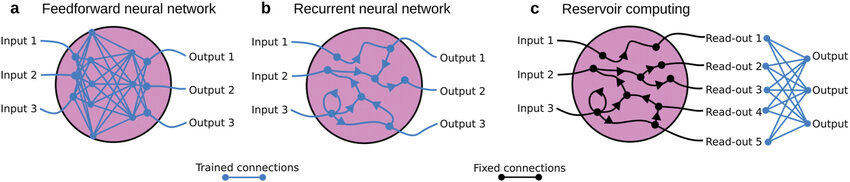
\includegraphics[width=0.7\textwidth]{figures/rc_difference_with others.png}
    \caption{RC vs traditional networks}
  \end{figure}
\end{frame}

\section{Basics of Reservoir Computing}
\begin{frame}{Core Architecture}
  \begin{columns}
    \column{0.6\textwidth}
    \begin{itemize}
      \item Three components:
      \begin{itemize}
        \item Input layer
        \item Reservoir (fixed random)
        \item Output layer (trained)
      \end{itemize}
      \item Discrete-time update:
      \[
      \mathbf{x}[n+1] = f(\mathbf{W}\mathbf{x}[n] + \mathbf{W}^{\text{in}}\mathbf{u}[n])
      \]
    \end{itemize}
    \column{0.4\textwidth}
    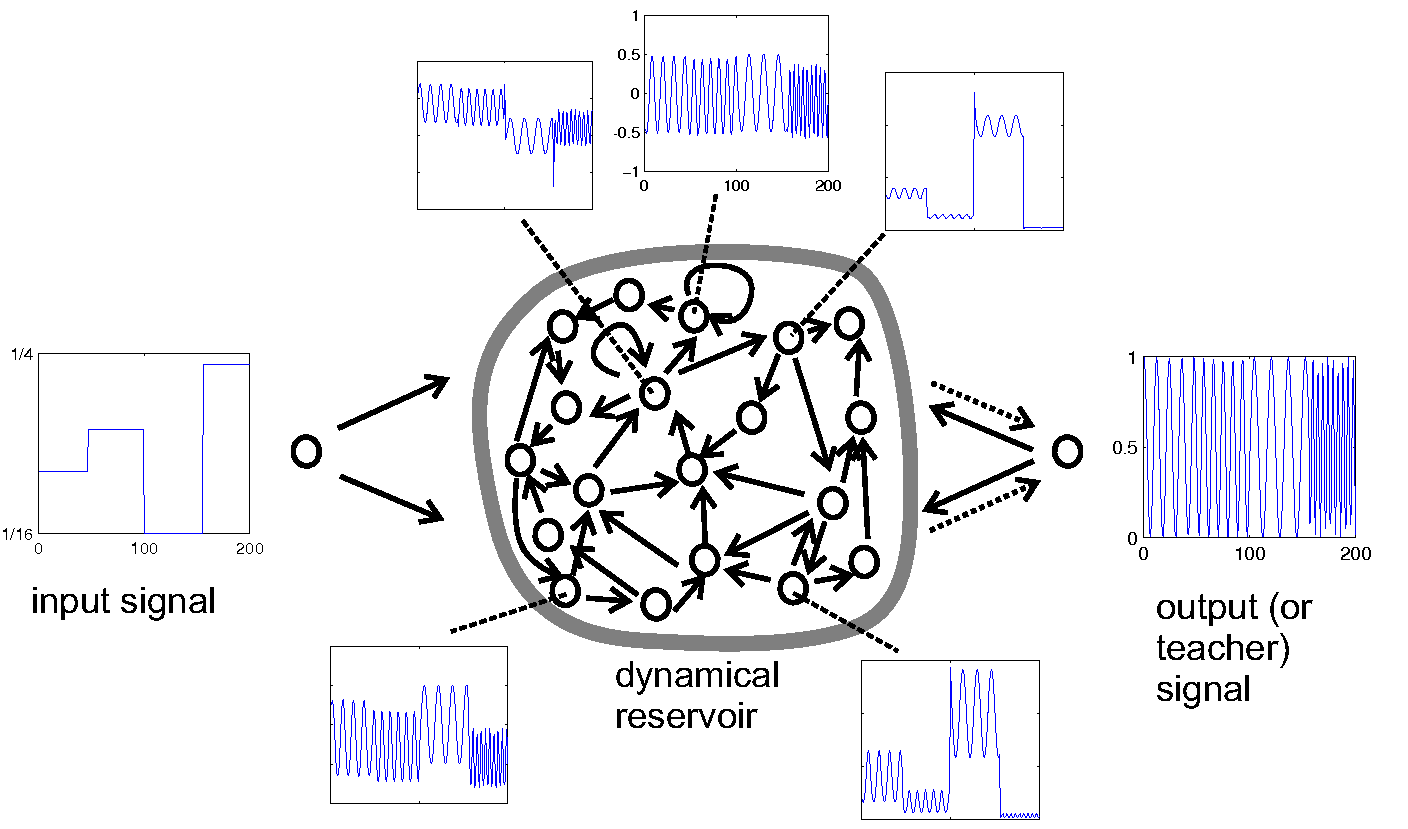
\includegraphics[width=\textwidth]{figures/ESN_diag_FreqGenSchema.png}
  \end{columns}
\end{frame}

\begin{frame}{Key Properties}
  \begin{block}{Echo State Property (ESP)}
    \begin{itemize}
      \item Fading memory concept
      \item Spectral radius < 1
      \item Input history dependence
    \end{itemize}
  \end{block}
  
  \begin{block}{Training Methodology}
    \[
    W_{\text{out}} = YG^T(GG^T + \lambda I)^{-1}
    \]
    Ridge regression for output weights
  \end{block}
\end{frame}

\begin{frame}{Variants and Comparisons}
  \begin{columns}
    \column{0.5\textwidth}
    \textbf{Variants:}
    \begin{itemize}
      \item Echo State Networks (ESN)
      \item Liquid State Machines (LSM)
      \item Physical Reservoirs
    \end{itemize}
    
    \column{0.5\textwidth}
    \textbf{vs Traditional RNNs:}
    \begin{itemize}
      \item Fixed reservoir vs full backprop
      \item Linear regression vs gradient descent
      \item Faster training
    \end{itemize}
  \end{columns}
  \vspace{5mm}
  \centering
  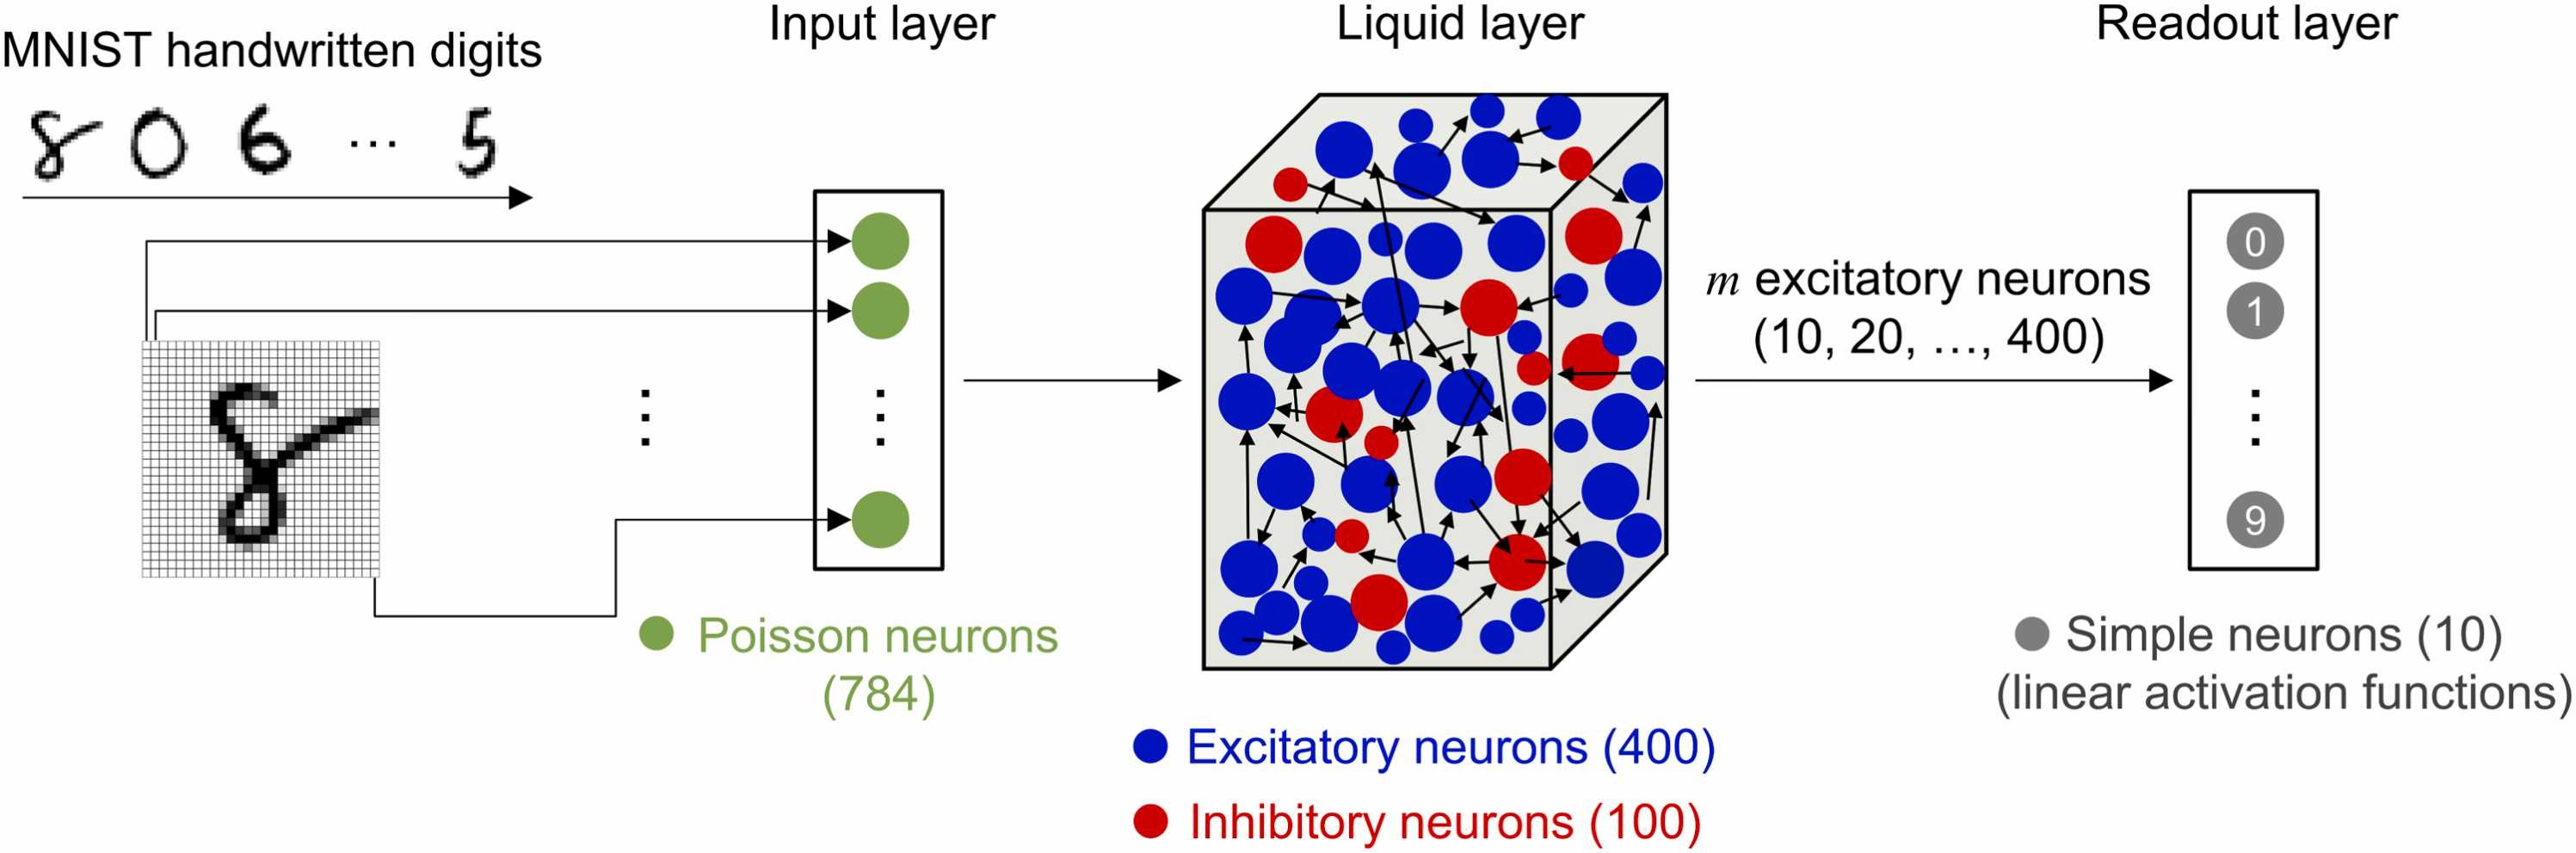
\includegraphics[width=0.4\textwidth]{figures/lsm_diag.png}
\end{frame}

\section{Implementations}
\begin{frame}{Pendulum Reservoir}
  \begin{columns}
    \column{0.6\textwidth}
    \begin{equation*}
      \begin{aligned}
        \frac{dx}{dt} &= v \\
        \frac{dv}{dt} &= -\frac{g}{l}\sin(x) - kv + f(t)
      \end{aligned}
    \end{equation*}
    \begin{itemize}
      \item Single nonlinear oscillator
      \item Angle and velocity as states
    \end{itemize}
    
    \column{0.4\textwidth}
    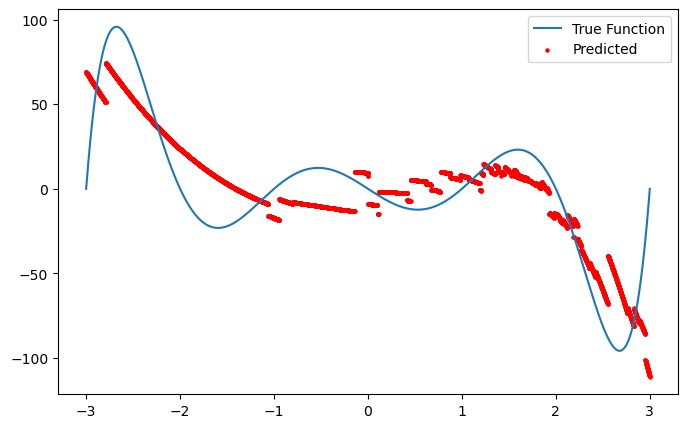
\includegraphics[width=\textwidth]{figures/pendulum_result_0.png}
  \end{columns}
\end{frame}

\begin{frame}{Lorenz System Prediction}
  \begin{columns}
    \column{0.5\textwidth}
    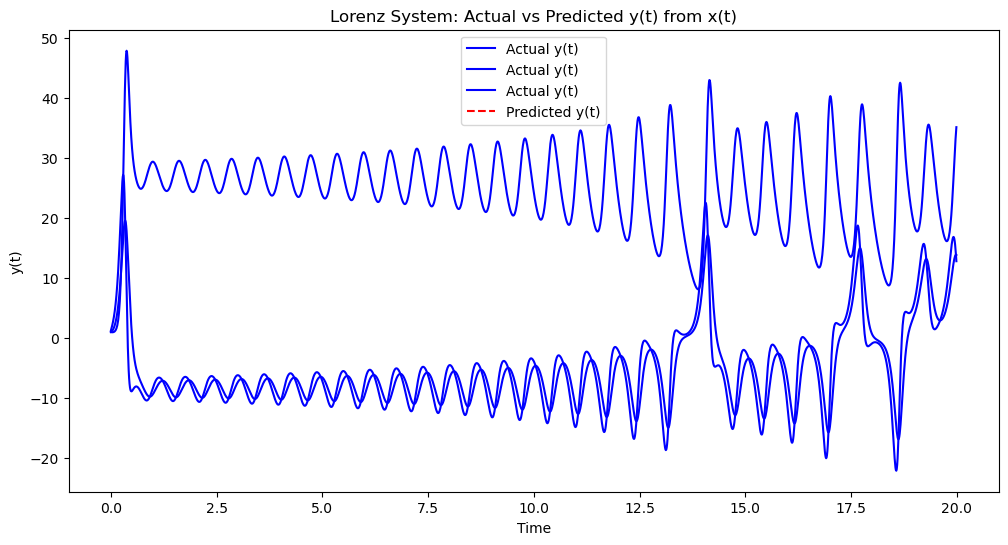
\includegraphics[width=\textwidth]{figures/lorentz_pendulum_1.png}
    
    \column{0.5\textwidth}
    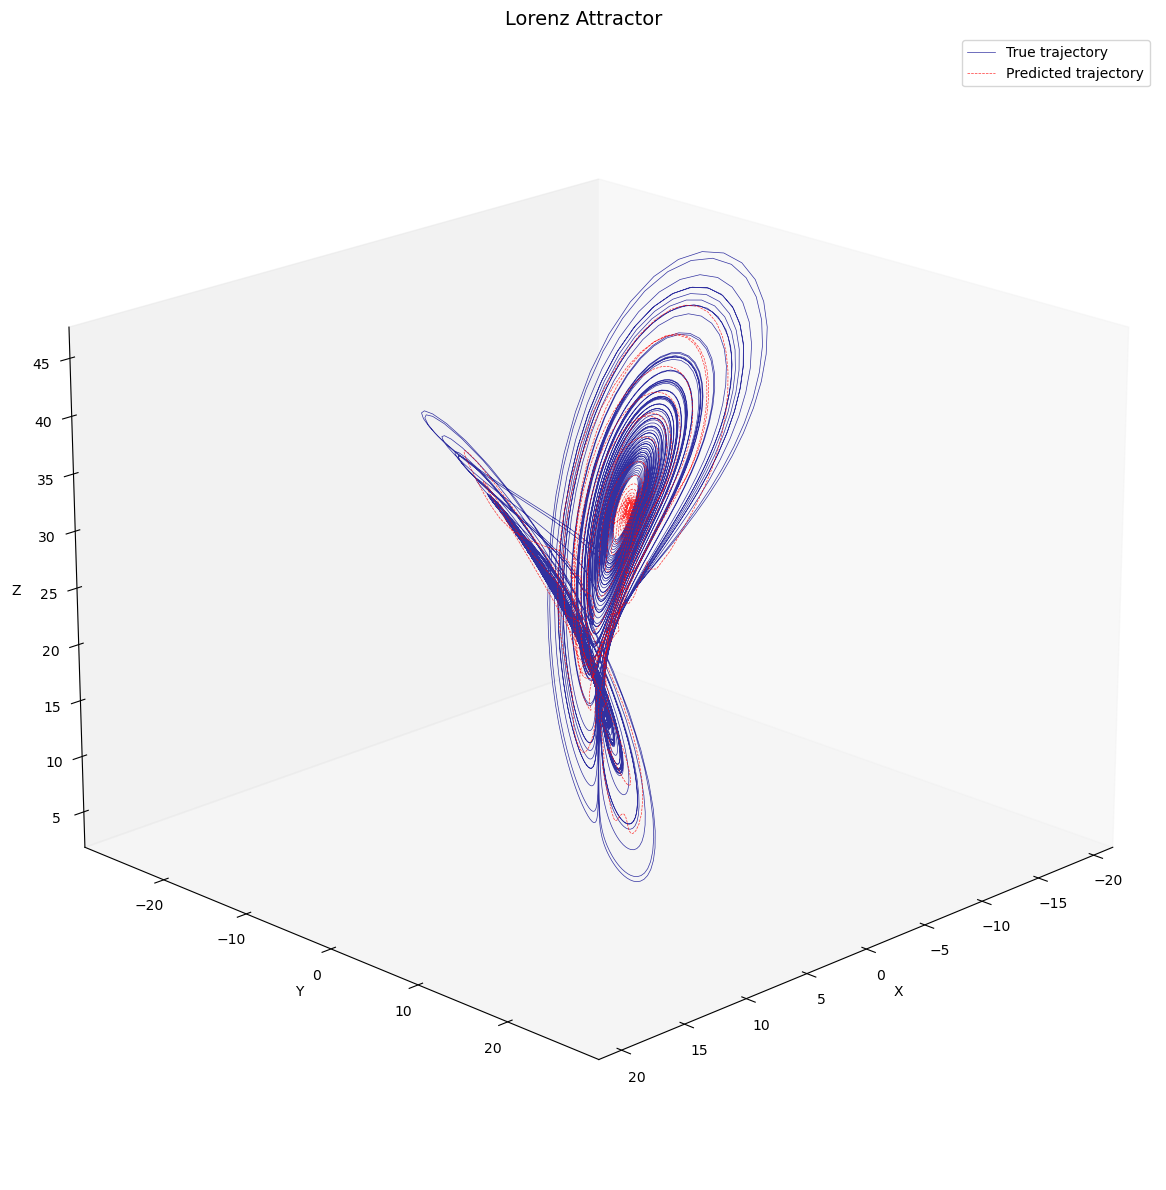
\includegraphics[width=\textwidth]{figures/lorentz_pendulum_2.png}
  \end{columns}
  \begin{center}
    RMSE: [3.77, 2.94, 8.36]
  \end{center}
\end{frame}

\begin{frame}{Logistic Map Reservoir}
  \begin{columns}
    \column{0.6\textwidth}
    \[
    x_{n+1} = rx_n(1-x_n)
    \]
    \begin{itemize}
      \item Virtual nodes technique
      \item 7th-degree polynomial prediction
    \end{itemize}
    
    \column{0.4\textwidth}
    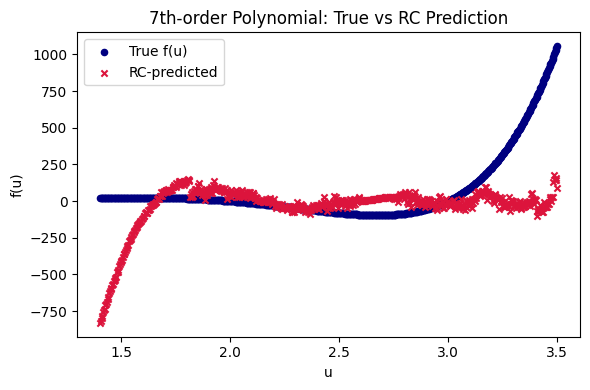
\includegraphics[width=\textwidth]{figures/logistic_7th_degree.png}
  \end{columns}
\end{frame}

\section{Bifurcation Analysis}
\begin{frame}{Reconstruction Pipeline}
  \begin{enumerate}
    \item Generate time-series for parameter range
    \item Train ELM on reservoir states
    \item Apply PCA on output weights
    \item Reconstruct bifurcation diagram
  \end{enumerate}
  \centering
  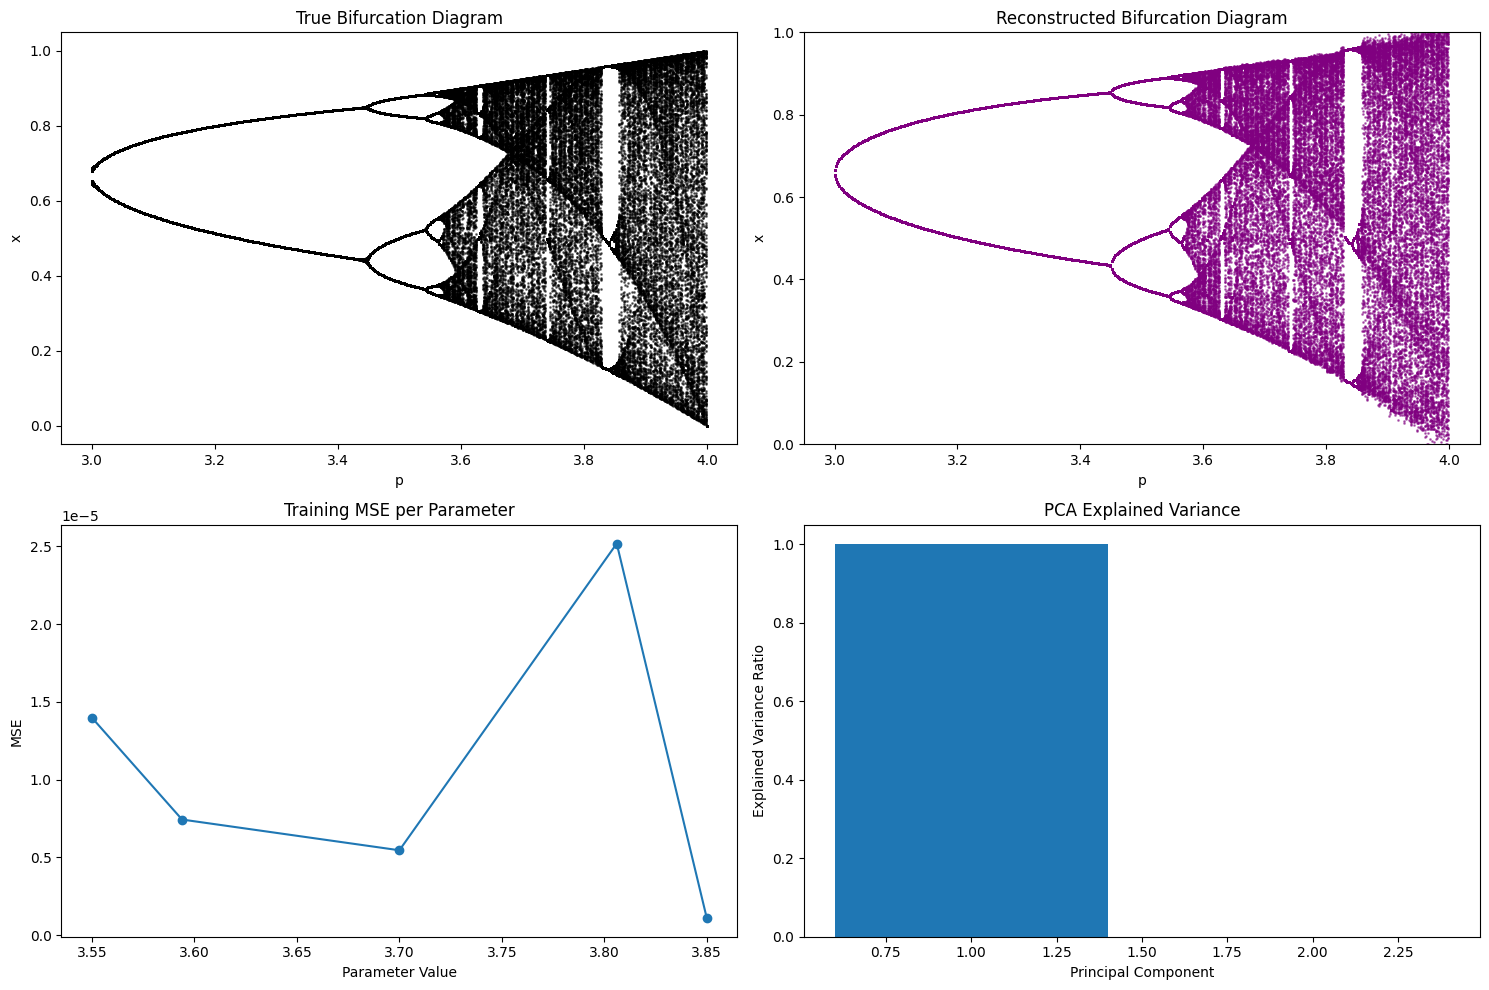
\includegraphics[width=0.6\textwidth]{figures/bd_1_results.png}
\end{frame}

\begin{frame}{Results Comparison}
  \begin{columns}
    \column{0.5\textwidth}
    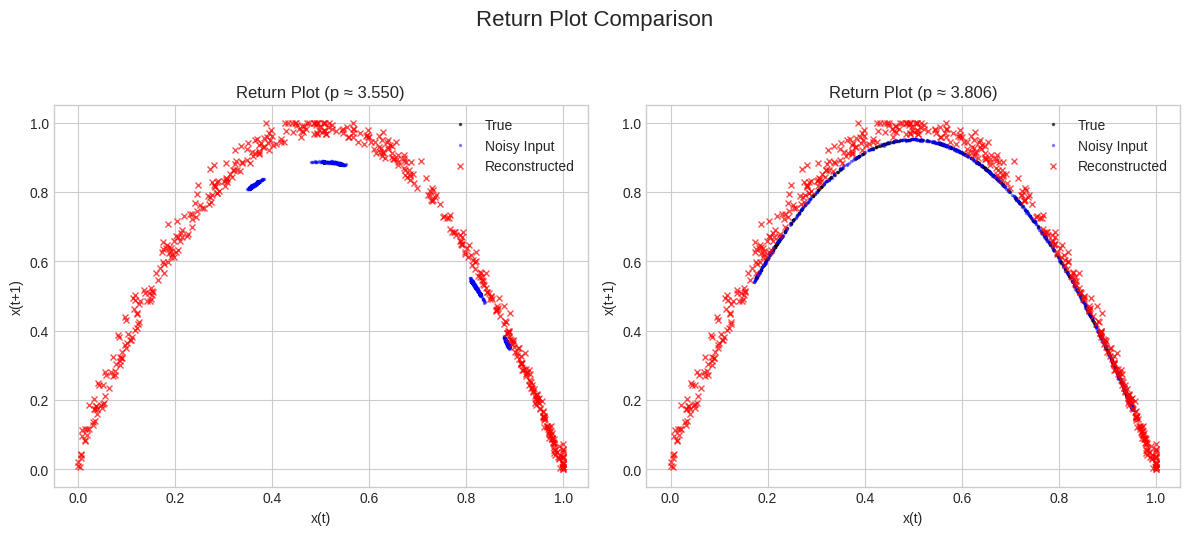
\includegraphics[width=\textwidth]{figures/bd_return_plot_2.png}
    
    \column{0.5\textwidth}
    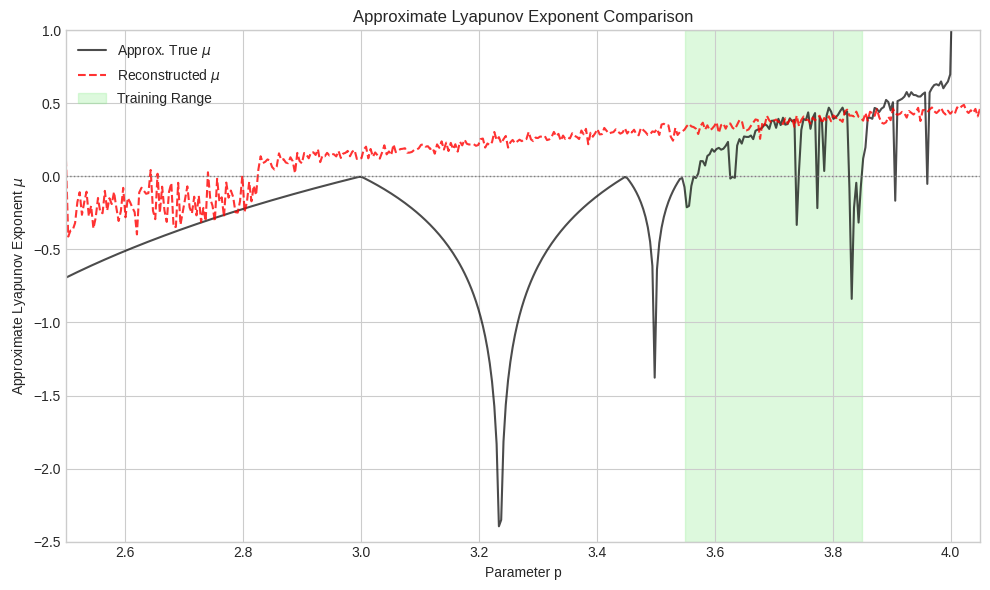
\includegraphics[width=\textwidth]{figures/lyapanov_bd_rd.png}
  \end{columns}
  \begin{center}
    Training MSE: 1.06e-05
  \end{center}
\end{frame}

\begin{frame}{LSTM Comparison}
  \begin{columns}
    \column{0.6\textwidth}
    \textbf{Advantages:}
    \begin{itemize}
      \item Explicit parameter input
      \item End-to-end training
      \item Better reconstruction
    \end{itemize}
    \textbf{Trade-off:}
    \begin{itemize}
      \item 46s vs <1s training
    \end{itemize}
    
    \column{0.4\textwidth}
    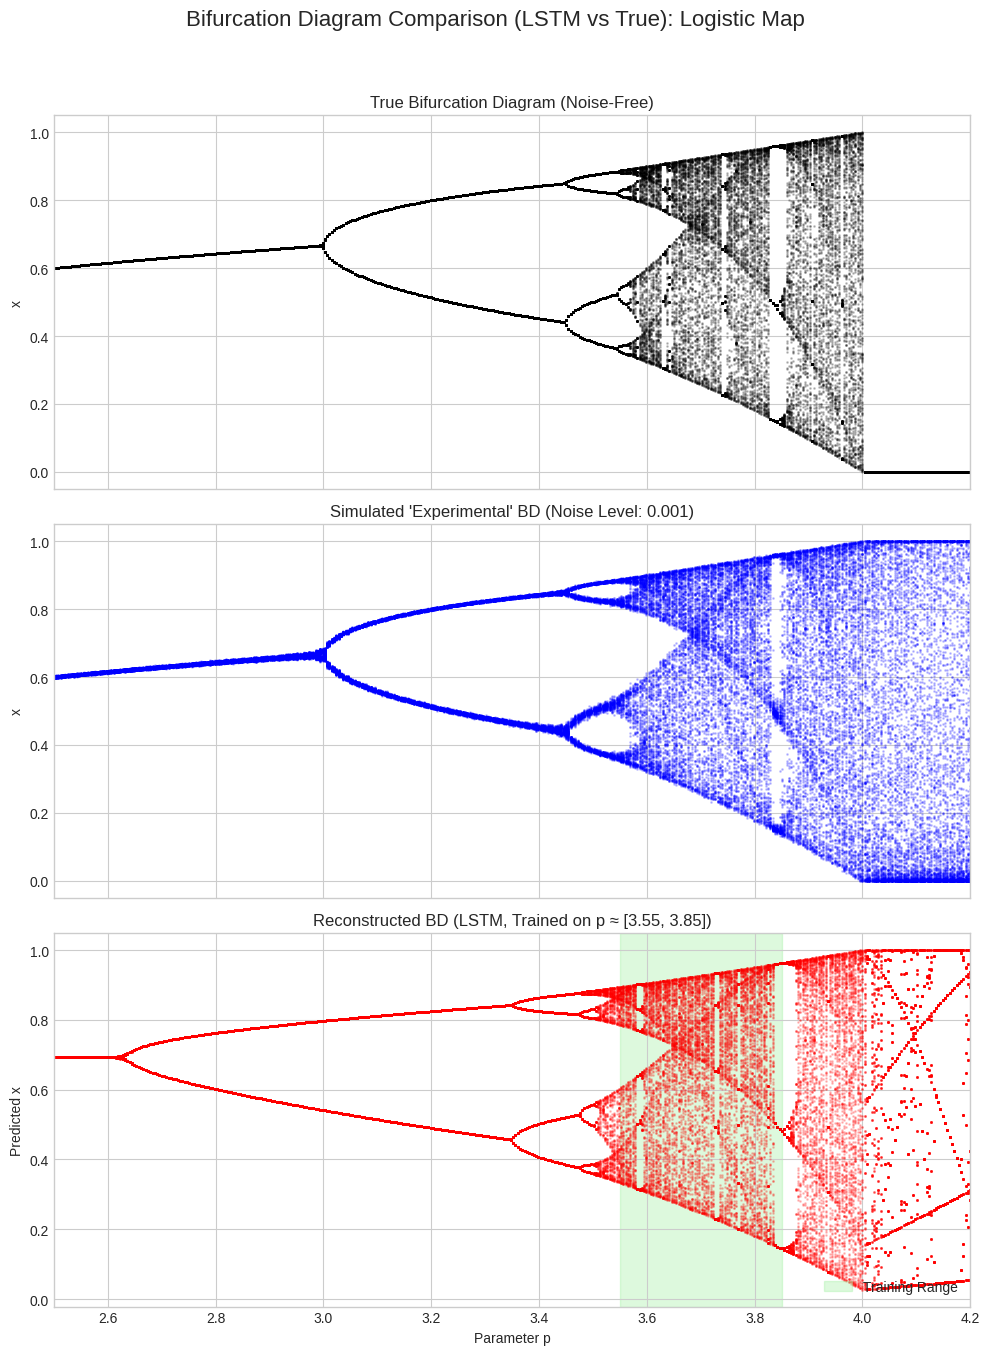
\includegraphics[width=\textwidth]{figures/lstm_bd_1.png}
  \end{columns}
\end{frame}

\section{Conclusion \& Future Work}
\begin{frame}{Key Takeaways}
  \begin{itemize}
    \item RC enables efficient temporal processing
    \item Physical systems can serve as reservoirs
    \item Successful bifurcation reconstruction
    \item Trade-offs between RC and LSTM
  \end{itemize}
  \vspace{5mm}
  \centering
  \includegraphics[width=0.5\textwidth]{figures/bd_3_results_overlapped.png}
\end{frame}

\begin{frame}{Future Directions}
  \begin{itemize}
    \item Hyperparameter optimization
    \item Extended system analysis:
    \begin{itemize}
      \item Higher-dimensional systems
      \item Different bifurcation types
    \end{itemize}
    \item Hardware implementation
    \item Hybrid architectures
  \end{itemize}
  \vspace{5mm}
  \centering
  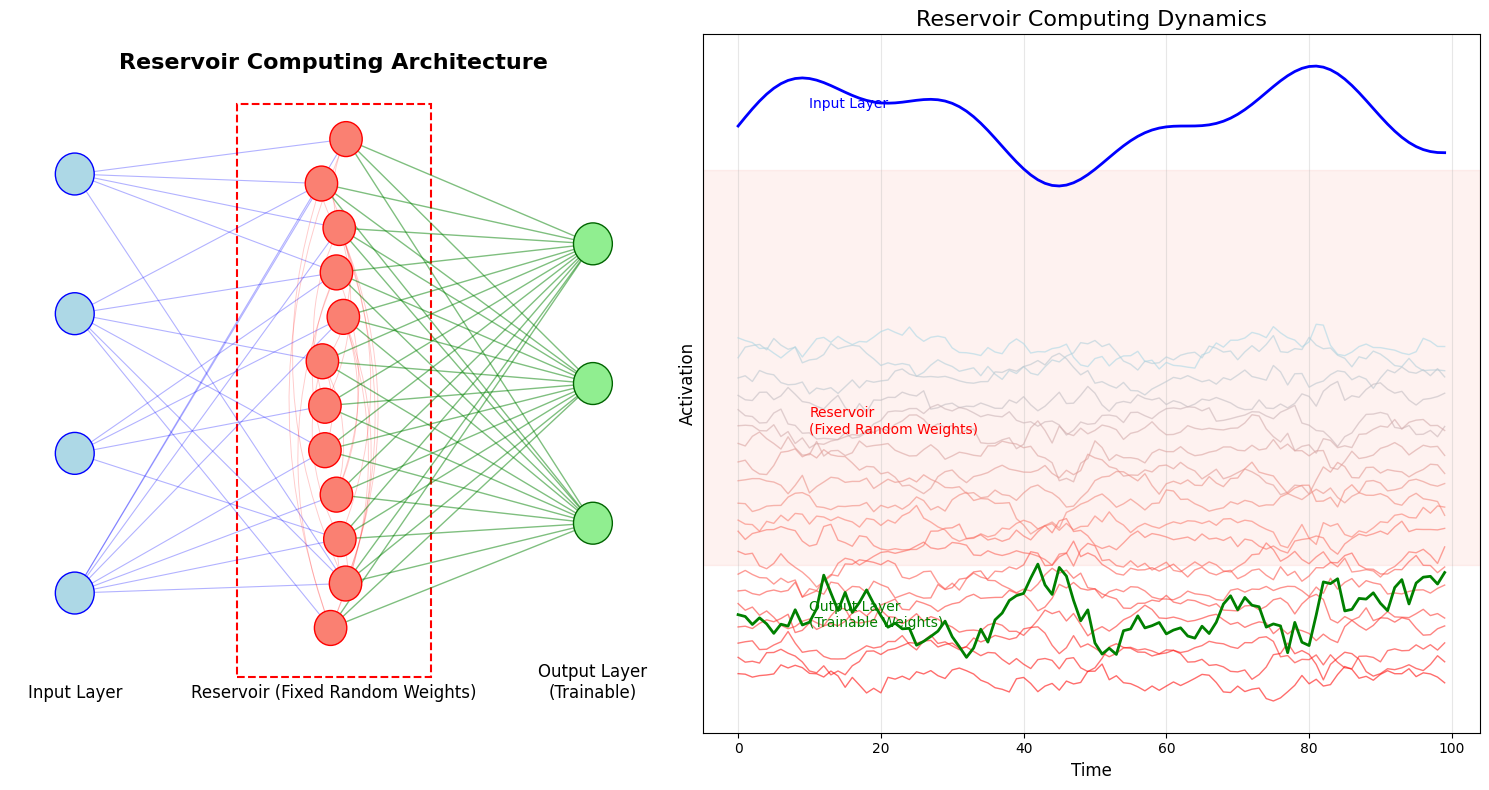
\includegraphics[width=0.4\textwidth]{ivt-style/rc_intro_matplotlib.png}
\end{frame}

\begin{frame}{Acknowledgements}
  \centering
  \Large
  Thank You!\\
  \vspace{1cm}
  Questions?\\
  \vspace{1cm}
  \small
  Code available at:\\
  \href{https://github.com/vimarsh244/ResorvoirComputing_SOP}{github.com/vimarsh244/ResorvoirComputing\_SOP}
  
  \vspace{0.5cm}
  Special thanks to Prof. Gaurav Dar
\end{frame}

\end{document}